\documentclass[10pt,twocolumn]{article}
\usepackage[letterpaper,margin=0.72in,columnsep=0.25in]{geometry}
\usepackage[T1]{fontenc}
\usepackage{lmodern}
\usepackage{amsmath,amssymb,booktabs,graphicx,microtype}
\usepackage{xcolor,tikz}
\usetikzlibrary{arrows.meta,positioning,fit,calc}
\usepackage[hidelinks]{hyperref}
\usepackage{url,flushend}
\hypersetup{pdftitle={MR-NWM: Language-Model-Centered World Models for Multimodal, Multi-Rate RAN Control},pdfauthor={},pdfsubject={Research preprint and reproducible synthetic benchmark},pdflang={en-US}}
\setlength{\parindent}{1em}
\setlength{\parskip}{0pt}
\setcounter{dbltopnumber}{3}
\renewcommand{\dbltopfraction}{0.85}
\newcommand{\R}{\mathbb{R}}
\newcommand{\E}{\mathbb{E}}
\newcommand{\sg}{\operatorname{stopgrad}}
\title{\vspace{-1.4em}MR-NWM: Language-Model-Centered World Models\\for Multimodal, Multi-Rate RAN Control}
\author{}
\date{Research preprint, October 2026}

\begin{document}
\maketitle
\begin{abstract}
MR-NWM is a language-model-centered architecture for multimodal, multi-rate
radio access network (RAN) world modeling. A pretrained language transformer
serves as the shared slow backbone. Continuous modality adapters receive
state/traffic sequences, real/imaginary CSI and IQ features, topology nodes,
and optional patch features, with explicit observation ages and sampling
periods. Two causal views of the same language backbone separate operational
preferences from exogenous physical evidence. A context-conditioned recurrent
subnetwork then predicts numerical state transitions at the fast rate using a
cached modulation packet, with optional slow/fast physics-expert sharing.
We supply this pretrained-model integration alongside a lightweight,
train-from-scratch reference variant. Three-seed, eight-variant measurements on
a fully specified two-link queue/interference simulator evaluate only the
lightweight variant: dynamics, distribution shift, controlled-language parsing,
action effects, decision regret, and host-observed timing. Those results do not
establish performance of a trained language-foundation RAN model. The project
provides executable multimodal/gradient/causality tests and a reproducible path
from the small reference experiment toward the intended language-based system,
without claiming calibrated radio behavior or deterministic real-time deadlines.
\end{abstract}

\section{Introduction}
Network operators express objectives in terms of service quality, energy,
reliability, and business priorities. A controller must translate these
objectives into measurable quantities, evaluate candidate actions against
network dynamics, and respect actuator and timing constraints. Language models
can provide an extensible interface to these tasks, while continuous-valued
predictors can represent the physical consequences of actions without
converting every measurement into text.

Two broad designs are possible: a common multimodal backbone can process
language and network measurements, or a semantic component can invoke a
separate dynamics model. Neither design inherently determines the numerical
representation of wireless observations. In particular, a language-derived
backbone can receive continuous embeddings, and a tool interface can transmit
continuous tensors. Nor does a modular interface necessarily prohibit joint
training: differentiability depends on the operations and training graph.
The relevant questions are therefore empirical: what should be shared, which
information should influence the transition law, and how should computational
work be divided across rates?

The full MR-NWM architecture places a pretrained language model at the center
of slow multimodal fusion and intent processing. Its numeric adapters and fast
physical subnetwork are jointly trainable around that backbone. The lightweight
reference hypothesis is that a slow context encoder and a small recurrent
transition operator can be coupled through weight sharing and low-dimensional
conditioning, while keeping intent-to-objective compilation explicit.
This construction builds on established multi-rate recurrence, hypernetworks,
feature modulation, and low-rank parameterization
\cite{koutnik2014,ha2016,perez2018,hu2022}. We do not claim these components
individually as new. The contribution of this reference study is their concrete
composition with an enforced preference/dynamics boundary and an evaluation
protocol that can falsify benefits from sharing or gradient coupling.

The implementation makes three choices that are particularly consequential.
First, continuous physical state and exogenous context enter through numeric
encoders rather than text quantization. Second, the slow physical stream cannot
read preference tokens, including through the recurrent expert. Third, a
forecast spanning two macro windows passes its predicted terminal state and
fast summary into the next window. Thus long-horizon errors cannot be hidden by
resetting the initial condition. These choices are independently covered by
regression tests.

\section{Language-Model-Centered Multimodal Architecture}
\subsection{Foundation and modality-specific encoders}
The full MR-NWM design uses a \emph{pretrained language transformer as the shared
slow backbone}. Continuous observations enter this backbone through trainable
modality adapters rather than being converted into strings. A separate fast
physical subnetwork performs the repeated numeric transitions between backbone
updates. This separation preserves a language-based foundation while assigning
high-frequency prediction to a smaller computational path.

\begin{figure*}[t]
\centering
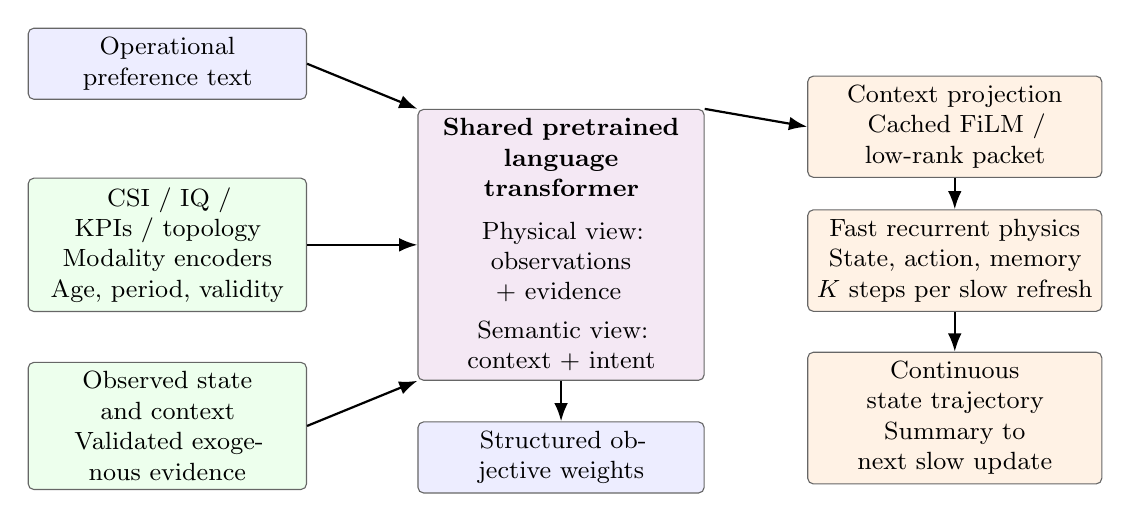
\begin{tikzpicture}[font=\small,>=Latex,
 box/.style={draw=black!60,rounded corners=2pt,align=center,minimum height=0.9cm},
 arr/.style={->,thick}]
 \node[box,fill=blue!7,text width=3.3cm] (intent) at (0,2.3)
 {Operational preference text};
 \node[box,fill=green!7,text width=3.3cm] (modal) at (0,0)
 {CSI / IQ / KPIs / topology\\Modality encoders\\Age, period, validity};
 \node[box,fill=green!7,text width=3.3cm] (evidence) at (0,-2.3)
 {Observed state and context\\Validated exogenous evidence};
 \node[box,fill=violet!9,text width=3.4cm,minimum height=3.1cm] (lm) at (5,0)
 {\textbf{Shared pretrained\\language transformer}\\[0.15cm]
 Physical view:\\observations + evidence\\[0.1cm]
 Semantic view:\\context + intent};
 \node[box,fill=orange!10,text width=3.5cm] (packet) at (10,1.5)
 {Context projection\\Cached FiLM / low-rank packet};
 \node[box,fill=orange!10,text width=3.5cm] (fast) at (10,-0.2)
 {Fast recurrent physics\\State, action, memory\\$K$ steps per slow refresh};
 \node[box,fill=blue!7,text width=3.4cm] (weights) at (5,-2.7)
 {Structured objective weights};
 \node[box,fill=orange!10,text width=3.5cm] (states) at (10,-2.2)
 {Continuous state trajectory\\Summary to next slow update};
 \draw[arr] (intent.east) -- (lm.north west);
 \draw[arr] (modal.east) -- (lm.west);
 \draw[arr] (evidence.east) -- (lm.south west);
 \draw[arr] (lm.north east) -- (packet.west);
 \draw[arr] (packet) -- (fast);
 \draw[arr] (fast) -- (states);
 \draw[arr] (lm.south) -- (weights.north);
\end{tikzpicture}
\caption{Language-centered architecture implemented by the foundation path. The
language transformer is the shared slow backbone; two separate views enforce the
preference/evidence boundary. Modality adapters and wireless heads require task
training. Fast predictions use the cached packet without calling the language model.}
\label{fig:language-foundation}
\end{figure*}

Let $x_T^{(m)}$ be observations of modality $m$, $v_T^{(m)}$ their validity mask,
$\delta_T^{(m)}$ their observation ages, and $\rho_m$ the acquisition period.
A modality encoder creates continuous tokens
\begin{equation}
 e_T^{(m)}=E_m(x_T^{(m)})+e_{\rm type}^{(m)}
       +E_{\rm time}[\log(1+\delta_T^{(m)}),\log(1+\rho_m)].
\end{equation}
The implementation supports variable token counts, explicitly masked missing
observations, and an input-token budget. A modality can be absent entirely.
Negative ages, non-finite valid measurements, and malformed masks are rejected.
These checks make the temporal information explicit; they are not a distributed
clock-synchronization or missing-data recovery system.

\begin{table*}[t]
\centering\small
\caption{Multimodal inputs in the language-foundation integration. Front ends are
trainable adapters; their radio representations require task-specific data and alignment.}
\begin{tabular}{p{0.16\textwidth}p{0.35\textwidth}p{0.40\textwidth}}
\toprule
Input & Representation entering the model & Implemented boundary and limitations\\
\midrule
Intent, protocol/evidence text & Language tokenizer IDs and masks & Preferences and exogenous evidence use separate typed fields.\\
State, traffic, KPIs & Continuous vectors or sequences & Numeric projections preserve values; timestamps and acquisition periods are supplied by the caller.\\
CSI and IQ & Continuous tokens with real/imaginary feature pairs & Linear/MLP adapters; complex preprocessing and RF calibration are external.\\
Topology & Node features and optional adjacency & One normalized graph message-passing step before language-backbone fusion.\\
Visual/map features & Continuous patch feature vectors & Configurable numeric patch adapter; raw-image patch extraction is external.\\
\bottomrule
\end{tabular}
\label{tab:modalities}
\end{table*}

For graph inputs, an optional normalized adjacency operator mixes neighboring
node embeddings before fusion. For CSI/IQ, the caller supplies explicit real
and imaginary components with known dimensions. Image or map patches can use
the same registered-adapter interface, but this release does not include a
pretrained vision encoder or raw-camera pipeline. Adapter presence alone does
not establish useful cross-modal alignment. That alignment must be learned and
tested on synchronized observation/action trajectories.

\subsection{Two views of one language backbone}
Physical predictions must be able to use information about the external world
without confusing it with the operator's preferences. The same pretrained
transformer $F_\theta$ therefore processes two separate input views. Let
\begin{equation}
 Z_T^p=[E_s(s_{T,0});E_c(c_T);E_H(H_{T-1});
                  \{e_T^{(m)}\}_m;E_K(K_T)],
\end{equation}
where $K_T$ contains externally supplied, validated evidence, such as an actual
configuration change. A learned query $q_p$ reads the physical view, while
intent tokens are appended only to the semantic view:
\begin{align}
 h_T^p&=P_pF_\theta([Z_T^p;q_p])_{\rm last},\\
 h_T^I&=P_IF_\theta([Z_T^p;E_I(I_T)])_{\rm last\ valid}.
\end{align}
Both views use the \emph{same language-model parameters}, with independent
forward passes and masks. Preferences cannot enter the physical forward pass
through attention or hidden-state reuse. By contrast, changes to observed
modalities or exogenous evidence may legitimately change predicted dynamics.
The caller is responsible for distinguishing a requested change from a change
that has actually been applied or externally observed.

The projected physical context passes through the recurrent physics expert and
then generates the fast-tier FiLM/low-rank packet. The physics expert can share
its parameters with the fast recurrence. This is a coupling around the language
trunk; the code does not claim to have converted the pretrained transformer's
internal feed-forward layers into wireless SSM experts. The objective head
uses $h_T^I$. Continuous state and structured objective heads are implemented;
general natural-language explanations and arbitrary protocol action decoders
remain additional output heads to develop and evaluate.

The \texttt{LanguageBasedWorldModel.from\_pretrained} entry point loads an actual
Hugging Face transformer checkpoint. A concrete small example is
\texttt{Qwen/Qwen2.5-0.5B} \cite{qwen2024}. Pretrained weights can be frozen while
gradients still propagate \emph{through} the transformer into numeric adapters.
Disabling autograd around the frozen trunk would break that training path and
is deliberately avoided. The numeric adapters, context projections, modulation
heads, and dynamics predictor start untrained; pretrained text weights do not
automatically provide a calibrated wireless world model.

\subsection{Multiple observation rates and execution rates}
The architecture distinguishes three quantities: each modality's acquisition
period $\rho_m$, the slow backbone's refresh interval $\Delta T$, and the fast
predictor's step interval $\Delta t$, with $\Delta T=K\Delta t$ in the basic
training graph. Observation tokens retain their own ages and periods even when
combined at one slow refresh. A token budget requires explicit pooling or
resampling before excessively long streams enter the language backbone.

Only two learned execution rates are implemented: one language-backbone update
per macro window and $K$ lightweight recurrent steps. Operator-level knowledge
retrieval, long-horizon task decomposition, and model lifecycle management can
run at a still slower external rate, but are not a third implemented neural
controller in this release. The fast API does not call the language backbone;
the contract tests count backbone calls to enforce this property.

Placement in Non-RT management, a Near-RT application, or an in-node predictor
depends on measured end-to-end budgets. No general language-model size or Python
module name establishes that placement. In particular, the language-foundation
version's latency must be measured separately from the lightweight prototype's
timing table. RF/CSI sampling, tensor fusion, model inference, network transport,
and actuator execution contribute different parts of the overall budget.

\subsection{What the two code paths establish}
The \texttt{foundation.py} path implements the intended language-centered
architecture and registered multimodal token adapters. Its tests cover causal
preference separation, graph/missing-data handling, input ages, frozen-trunk
gradient flow, and cached fast execution. The optional integration script records
the checkpoint identity and resolved revision. We executed this check with
Qwen2.5-0.5B on CPU, loading 494,032,768 pretrained backbone parameters and
connecting CSI, IQ, and topology feature tokens. The five-step output had shape
$1\times5\times6$; numeric-adapter gradients were nonzero with frozen backbone
weights, and preference changes left physical predictions unchanged. The record
is stored in \texttt{pretrained\_integration.json}. This establishes
software/gradient compatibility rather than a trained RAN model or a general
language-understanding score.

The following lightweight variant replaces the expensive language trunk with
small train-from-scratch attention/MLP components. Its controlled experiments
isolate recurrent dynamics, sharing, and modulation at low cost. The numerical
results later in this paper belong \emph{only} to that lightweight variant.
They are not evaluations of Qwen or evidence that language pretraining improves
wireless prediction.


\section{Related Work and Scope}
World models learn action-conditioned transitions for prediction and planning;
DreamerV3 is an influential example of learning control through a latent world
model across diverse environments \cite{hafner2023}. MR-NWM is a supervised
prediction and finite-candidate auditing study. It does not implement Dreamer,
learn an actor, or demonstrate reinforcement-learning performance.

Clockwork recurrent networks demonstrate that recurrent computation can be
partitioned by update frequency \cite{koutnik2014}. HyperNetworks generate
parameters for another network \cite{ha2016}; FiLM conditions computation with
feature-wise affine transformations \cite{perez2018}. LoRA parameterizes an
update using low-rank factors \cite{hu2022}. Here the low-rank factors are
generated from each macro context, while the base model is also trained.
This differs from the standard frozen-backbone fine-tuning setup of LoRA.

Input-dependent state-space models motivate selective recurrent memory
\cite{gu2023}. Our physics expert is a simple gated recurrence, with bounded
forgetting coefficients. It is neither an implementation of Mamba nor a
physics-constrained channel model. Similarly, the heterogeneous expert mixture
executes every expert and therefore offers no sparse-MoE compute saving.

Flow matching regresses a vector field along a prescribed probability path
\cite{lipman2023}. Transfusion provides an example of combining discrete and
continuous objectives in one multimodal model \cite{zhou2024}. We include an
optional action-conditioned flow head for future stochastic trajectory studies,
but the reported deterministic benchmark does not use it. In particular, no
claim about improved uncertainty calibration follows from its presence.

The repository has two explicit realizations. The language-foundation path
loads an external pretrained transformer and tokenizer and adds numeric/graph
adapters. The lightweight benchmark path uses randomly initialized semantic
MLPs, with no pretrained language weights. No over-the-air measurements, RIC
integration, or DU deployment are supplied. The controlled-language benchmark
cannot support open-domain or foundation-model zero-shot claims.

\section{Problem Formulation}
\subsection{State, actions, context, and intent}
Let $s_t\in\R^{d_s}$ denote the observable network state, $a_t\in\R^{d_a}$ a
candidate action, and $c_T\in\R^{d_c}$ measured exogenous context for macro
window $T$. Each window contains $K$ micro steps. Operational intent $I_T$
determines objective weights $w(I_T)$ and, in a fuller system, explicit
constraints. A causal transition model has the form
\begin{equation}
 s_{t+1}=F(s_t,a_t,c_T,\epsilon_t),\qquad
 U_t=w(I_T)^\top\psi(s_{t+1},a_t).
 \label{eq:causal}
\end{equation}
The preference part of an intent does not directly enter $F$. If a language
input reports an external event or a configuration change that affects
dynamics, that information must be extracted into a distinct, validated
context variable. If an intent changes the policy, it can of course change the
realized future \emph{through actions}. Equation~\eqref{eq:causal} concerns
predictions under the same intervened action sequence and context.

This separation gives a testable invariant:
\begin{equation}
 \hat{s}_{1:H}(I,a_{0:H-1},c,s_0)
 =\hat{s}_{1:H}(I',a_{0:H-1},c,s_0).
 \label{eq:invariant}
\end{equation}
The reference simulator satisfies this invariant by construction. A physical
event described in text is not interchangeable with an optimization preference;
keeping them in a single undifferentiated prompt would make the intended causal
semantics ambiguous.

\subsection{Time scales and placement}
Our notation describes computational rates, not measured radio deadlines.
The O-RAN architecture specifies Near-RT RIC control loops on the order of
10~ms to 1~s and permits faster control inside E2 nodes; loop timing is use-case
dependent \cite{oran2026}. A sub-millisecond fast model is a possible engineering
target for selected functions, rather than a consequence of assigning a module
to a DU. Likewise, $K$ is a modeling hyperparameter here; no micro-step in the
toy simulator is calibrated to a transmission interval.

\section{Lightweight Reference Variant and Training}
\subsection{Slow heterogeneous mixture}
At each macro step, token embeddings for intent, a state projection, a context
projection, and the previous fast summary form
\begin{equation}
 Z_T=[E_I(I_T);E_s(s_{T,0});E_c(c_T);H_{T-1}].
\end{equation}
The intent tokenizer is fitted only to the controlled training corpus. Learned
positions are added to intent tokens; physical token types have their own
encoders. A single attention block produces $h_i$, followed by a dense mixture
of one semantic MLP expert $E_{\rm sem}$ and one recurrent expert
$E_{\rm phy}$. For a modality indicator $m_i$,
\begin{align}
 \pi_i &=\operatorname{softmax}(W_g[h_i;\operatorname{onehot}(m_i)]),\\
 y_i &=\pi_{i,\rm sem}E_{\rm sem}(h_i)
       +\pi_{i,\rm phy}E_{\rm phy}(h_i).
\end{align}
For intent tokens the physics term is the identity, and the recurrent physics
expert starts afresh at the first physical token. Physical attention queries
are masked from intent keys. Both restrictions are necessary: attention masking
alone would still allow a recurrent expert to carry semantic information into
physical tokens. The semantic stream may read the physical context.

The mean physical output gives $h_T^p$. A masked mean over intent outputs gives
$h_T^I$, and a head predicts
$\hat w_T=\operatorname{softmax}(W_I h_T^I)$ over throughput, queue, and energy
features. The router is weakly regularized by
\begin{equation}
 \mathcal L_{\rm route}=-\frac{1}{|\mathcal V|}
 \sum_{i\in\mathcal V}\log\pi_{i,m_i},
\end{equation}
where $\mathcal V$ excludes padding. This encourages modality specialization;
it does not establish that the experts learn interpretable physical laws.

\begin{figure*}[t]
\centering
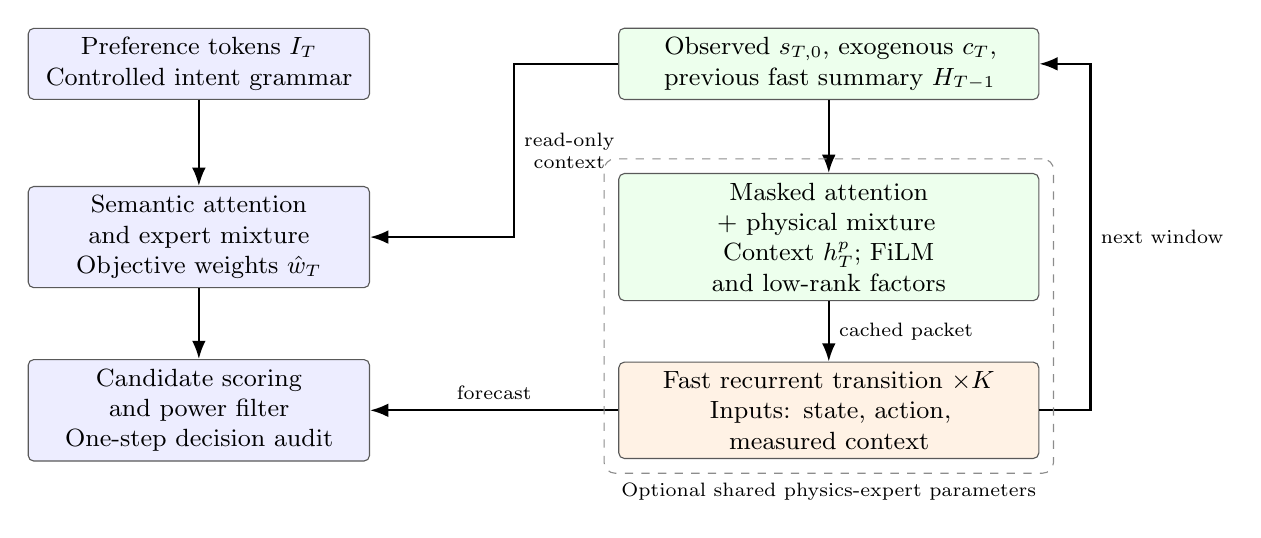
\begin{tikzpicture}[
 font=\small,>=Latex,
 box/.style={draw=black!65,rounded corners=2pt,align=center,minimum height=0.85cm},
 arr/.style={->,thick},node distance=0.45cm]
 \node[box,fill=blue!7,text width=4.1cm] (intent) at (0,2.6)
 {Preference tokens $I_T$\\Controlled intent grammar};
 \node[box,fill=green!7,text width=5.1cm] (physical) at (8,2.6)
 {Observed $s_{T,0}$, exogenous $c_T$,\\previous fast summary $H_{T-1}$};
 \node[box,fill=blue!7,text width=4.1cm] (sem) at (0,0.4)
 {Semantic attention\\and expert mixture\\Objective weights $\hat w_T$};
 \node[box,fill=green!7,text width=5.1cm] (slow) at (8,0.4)
 {Masked attention + physical mixture\\Context $h_T^p$; FiLM and low-rank factors};
 \node[box,fill=orange!10,text width=5.1cm] (fast) at (8,-1.8)
 {Fast recurrent transition $\times K$\\Inputs: state, action, measured context};
 \node[box,fill=blue!7,text width=4.1cm] (utility) at (0,-1.8)
 {Candidate scoring\\and power filter\\One-step decision audit};
 \draw[arr] (intent) -- (sem);
 \draw[arr] (physical) -- (slow);
 \draw[arr] (physical.west) -- (4,2.6) -- node[right,align=center,font=\scriptsize]
 {read-only\\context} (4,0.4) -- (sem.east);
 \draw[arr] (sem) -- (utility);
 \draw[arr] (slow) -- node[right,font=\scriptsize] {cached packet} (fast);
 \draw[arr] (fast) -- node[above,font=\scriptsize] {forecast} (utility);
 \draw[arr] (fast.east) -- ++(0.65,0) |- node[pos=0.25,right,font=\scriptsize]
 {next window} (physical.east);
 \node[draw=black!45,dashed,rounded corners,fit=(slow)(fast),inner sep=0.18cm,
 label={[font=\scriptsize]below:Optional shared physics-expert parameters}] {};
\end{tikzpicture}
\caption{Lightweight reference-variant information flow. Physical prediction has no path from preference
tokens. The semantic stream can use physical observations; numerical action evaluation
uses the forecast and compiled objectives. Slow and fast execution are separated in the
API, while shared training parameters remain a research option.}
\label{fig:architecture}
\end{figure*}

\subsection{Fast recurrence and modulation}
A hyper-projection from $h_T^p$ generates
$(\gamma_T,\beta_T,A_T,B_T)$, with
$\gamma_T=1+0.1\tanh(\cdot)$,
$\beta_T=0.1\tanh(\cdot)$, and bounded factors $A_T,B_T\in\R^{d\times r}$.
Within a macro window, these tensors are held fixed. Each micro step encodes
the current state, candidate action, and measured context:
\begin{equation}
 x_k=\gamma_T\odot\operatorname{SiLU}(W_x[s_k;a_k;c_T])+\beta_T.
\end{equation}
Let $n_k=\operatorname{LN}(x_k)$ and
$(u_k,g_k)=W_{\rm in}n_k$, with a SiLU applied to $u_k$. The physics memory is
\begin{align}
 \alpha_k&=\sigma(W_\alpha u_k),\\
 z_k&=\alpha_k\odot z_{k-1}+
        (1-\alpha_k)\odot\tanh(W_Bu_k),\\
 o_k&=x_k+W_o[W_Cz_k\odot\sigma(g_k)]
           +\frac{n_kA_TB_T^\top}{\sqrt r},\\
 \hat s_{k+1}&=\hat s_k+W_\Delta o_k.
 \label{eq:fast}
\end{align}
The last expression is a residual \emph{state increment}; the measured state is
not replaced by an action-independent macro forecast. Although $z_k$ has a
bounded convex update, this alone does not guarantee stability of the complete
autoregressive predictor or the downstream control loop.

In the shared variant, the slow physical expert and fast recurrence refer to
the identical parameter object. No extra copy is trained. A separately deployed
process would instead receive a versioned copy of the trained parameters;
weight sharing during training does not create cross-machine shared memory.
The unshared variant allocates an independent fast core. All variants retain
explicit dependence on actions and continuous context.

\subsection{Feedback and training graph}
The $K$ fast hidden states are compressed by a kernel-$K$, stride-$K$ one-dimensional
convolution into $H_T$. This summary is available to the \emph{next} macro step.
It cannot contain future observations. Memory $z$ resets at a macro boundary;
information persists through $H_T$ and the terminal predicted state.

Training uses two consecutive macro windows, initialized once with the observed
state. At the boundary,
\begin{equation}
 s_{T+1,0}=\hat s_{T,K},\qquad
 H_T=R(o_{T,1:K}).
\end{equation}
No target state is substituted. Within each macro window, $s_k$ and $z_k$ are
detached every $L=3$ steps. The modulation tensors retain their gradients.
The direct path from each micro-step loss to the slow context therefore remains
available despite truncation. Shared parameters also receive gradients through
the fast recurrence itself. Truncation limits the differentiated history; it
neither proves convergence nor prevents all gradient explosions. We additionally
clip the global gradient norm to one.

With $H=2K$, the reference loss is
\begin{align}
 \mathcal L&=\mathcal L_{\rm dyn}+0.2\mathcal L_I+0.01\mathcal L_{\rm route},\\
 \mathcal L_{\rm dyn}&=\frac{1}{BHd_s}\sum_{b,k,j}
    (\hat s_{b,k,j}-s_{b,k,j})^2,\\
 \mathcal L_I&=-\frac{1}{2B}\sum_{b,T,j}w_{b,j}\log\hat w_{b,T,j}.
\end{align}
Semantic targets are determined by the actual words in each training phrase.
There is no independently sampled next-token target and no claim of language
model pretraining. The optional flow loss is disabled for all reported runs.

For a controlled gradient ablation, the detached variant uses an independent
fast core and $\sg(h_T^p)$ before its modulator. The modulator, fast core,
semantic head, and route loss remain trainable. Comparing this variant with
the \emph{unshared} jointly trained model isolates the bridge-gradient choice.
Comparing it only with the shared model would also change parameter sharing.

\subsection{Optional probabilistic trajectory head}
For an optional extension, let $y=s_{T,1:K}$ and
$\xi\sim\mathcal N(0,I)$. A velocity network conditioned on both $h_T^p$ and the
\emph{candidate action sequence} minimizes
\begin{equation}
 \E_{\tau,\xi}\big\|v_\phi((1-\tau)\xi+\tau y,\tau,h_T^p,a_{0:K-1})
                         -(y-\xi)\big\|^2.
\end{equation}
The sampling API requires an explicit base draw and integrates the velocity
using Euler steps. Starting every sample at zero would not reproduce the
Gaussian-base generative model. The optional output is separate from
Equation~\eqref{eq:fast}; it is not silently injected into the deterministic
rollout. We test differentiation and sampling reproducibility, while leaving
probabilistic accuracy and calibration for a dedicated study.

\section{Reproducible Evaluation Protocol}
\subsection{Normalized two-link environment}
The state contains two link gains $g$, two queues $q$, and two interference
variables $j$. Actions are two normalized powers $p\in[0,1]^2$; context contains
arrival rates $\lambda_1,\lambda_2$, cross-coupling $\chi$, and mobility $\mu$.
For each link $i$, with $\bar i$ its neighbor,
\begin{align}
 g'_{i}&=\operatorname{clip}((1-\mu)g_i+0.55\mu+\epsilon_i,0.05,1.2),\\
 r_i&=\log_2\left(1+\frac{4g_ip_i}{0.2+j_i+\chi p_{\bar i}}\right),\\
 q'_i&=\operatorname{clip}(q_i+\lambda_i-0.12r_i,0,2),\\
 j'_i&=0.65j_i+0.35\chi p_{\bar i},
\end{align}
where $\epsilon_i\sim\mathcal N(0,0.005^2)$. Powers are independently sampled
uniformly on $[0,1]$. Initial gains, queues, and interference are uniformly
sampled from $[0.2,0.9]$, $[0.1,0.9]$, and $[0.05,0.25]$, respectively.
Training context uses $\lambda_i\sim U(0.05,0.15)$,
$\chi\sim U(0.08,0.25)$, and $\mu\sim U(0.03,0.12)$.
The joint shift adds $0.12$, $0.30$, and $0.25$ to those variables, respectively.
Thus OOD context values for coupling and mobility do not overlap training.

The system has controllable queues and delayed interference, but no waveform,
antenna array, coding, beam management, scheduler, packet simulator, or calibrated
propagation model. It is an intentionally small system-identification test.
The coefficients and state normalization are synthetic choices; they must not
be interpreted as measurements of a mobile network.

\subsection{Intent splits and decision audit}
Three objective names---throughput, latency, and energy---are used in singleton
and two-objective phrases. A target puts equal weight on the named objectives.
Three training templates vary the wording. Two held-out templates reorder the
same known words. An additional test uses all three objectives together, a
combination absent during training. No model or tokenizer is fitted to these
test phrases. Because this is a deliberately constrained grammar, its scores
measure compositional parsing under that grammar, not open-language zero-shot
generalization.

For each test state we also enumerate powers from
$\{0.1,0.4,0.7\}^2$, retaining only candidates with
$p_1+p_2\leq0.8$. The utility features are normalized post-transition rate,
negative mean queue, and negative mean power. The learned model chooses a
candidate using predicted features and inferred weights. We measure the regret
against the exact simulator's best \emph{feasible candidate}, evaluated with
the true intent weights. A second regret calculation substitutes the true
weights into model selection to isolate prediction error from parsing error.
The audit is deterministic and one step long; it is not a learned policy or
an end-to-end closed-loop control experiment. Zero power violations are an
expected property of the candidate filter, not evidence of learned safety.

\subsection{Baselines and matched comparisons}
The eight executable variants are: shared MR-NWM; unshared MR-NWM; shared MR-NWM
without FiLM or low-rank modulation; the unshared detached-bridge control; an
action/context-conditioned residual MLP; an approximately parameter-matched MLP;
a standalone recurrent model; and persistence. The MLPs have two hidden layers
of width 64 and 160, respectively, and predict the same state increments. They have no
semantic parser, so semantic scores are not invented for that baseline.
The standalone recurrent control uses the same fast recurrence and truncation
schedule as MR-NWM, with no slow tier or modulation. Parameters and optimization
steps are reported rather than claiming exact compute matching. No pure LLM,
pretrained wireless foundation model, or
industrial controller is represented by a synthetic row in a table.

All trainable variants use 300 AdamW updates, batch size 48, learning rate 0.002,
and weight decay $10^{-4}$. MR-NWM uses width 32, recurrent state size 16, rank 2,
four attention heads, and $K=5$. All models receive identical training
trajectories, indexed by seeds $100000+u$ for update $u$. Initialization seeds
are 11, 22, and 33. Evaluation uses 256 trajectories per split with seed
900000, never used for training. Models are evaluated after the fixed final
update; no test score selects a checkpoint or changes the budget.

\subsection{Metrics and timing}
We use signal-energy NMSE,
\begin{equation}
 10\log_{10}\frac{\sum_{b,k,j}(\hat s_{b,k,j}-s_{b,k,j})^2}
                      {\sum_{b,k,j}s_{b,k,j}^2},
\end{equation}
with lower values better. This is distinct from dividing MSE by centered
target variance. Per-step MSE and per-state NMSE accompany the aggregate,
since a global score can hide errors in small-scale variables. A paired action
audit compares the predicted trajectory difference under $a$ and $1-a$ with
the noise-free simulator difference. A predictor ignoring actions has zero
effect and therefore an action-effect NMSE of 0~dB.

Intent parsing uses total variation distance
$\tfrac12\|\hat w-w\|_1$ and cosine similarity. Cosine is not converted into
an invented ``alignment percentage.'' For latency, the model is in inference
mode; measurements use ten warm-up calls followed by 100 timed batch-one calls,
with device synchronization around timed regions. We retain raw timing samples
and report p50, p95, and p99. The fast measurement uses a cached modulation packet
and a supplied recurrent state. It excludes slow encoding, data acquisition,
transport, scheduling, model loading, and actuator execution. It therefore
cannot establish a radio control deadline or a deterministic worst-case bound.

\section{Results and Interpretation}
\begin{table*}[t]
\centering
\caption{Measured signal-energy NMSE over ten consecutive forecast steps. Values are
mean $\pm$ sample standard deviation over three initialization seeds. All rows
use the same held-out physical trajectories for a given dynamics split.}
\label{tab:results}
\begin{tabular}{lrrr}
\toprule
Model & Parameters & IID NMSE (dB) & OOD NMSE (dB) \\
\midrule
MR-NWM shared & 28,031 & -22.24 $\pm$ 0.20 & -9.58 $\pm$ 0.41 \\
MR-NWM unshared & 32,815 & -21.99 $\pm$ 1.13 & -9.34 $\pm$ 0.86 \\
No modulation & 28,031 & -21.64 $\pm$ 0.15 & -9.47 $\pm$ 0.88 \\
Detached bridge & 32,815 & -21.63 $\pm$ 0.96 & -9.56 $\pm$ 0.99 \\
Residual MLP & 5,382 & -14.36 $\pm$ 0.07 & -6.33 $\pm$ 0.23 \\
Matched-size MLP & 28,806 & -14.92 $\pm$ 0.35 & -7.15 $\pm$ 0.70 \\
Standalone recurrent & 5,398 & -21.19 $\pm$ 0.30 & -9.43 $\pm$ 0.37 \\
Persistence & 0 & -3.67 $\pm$ 0.00 & -6.87 $\pm$ 0.00 \\
\bottomrule
\end{tabular}

\end{table*}

\begin{figure*}[t]
\centering
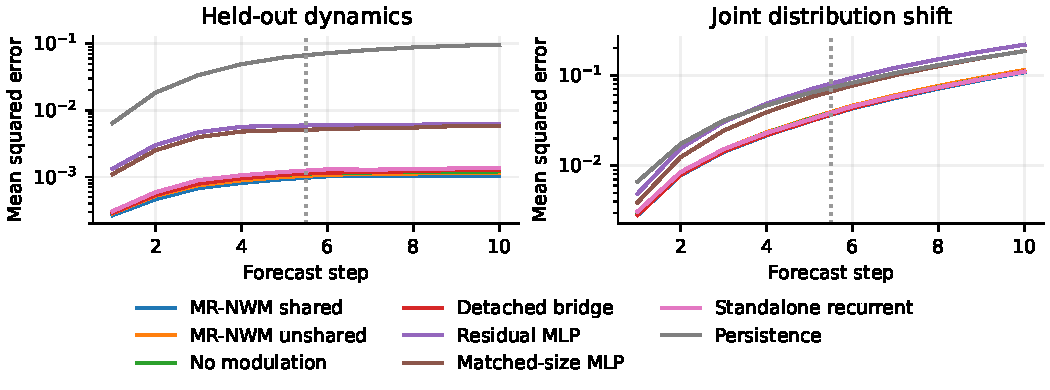
\includegraphics[width=0.92\textwidth]{figures/rollout_error.pdf}
\caption{Measured forecast error by horizon. The dotted boundary separates two
five-step macro windows; the second window starts from the model's first-window
terminal prediction. Curves average three initialization seeds. Raw per-seed
curves and per-state NMSE are retained in the result manifest.}
\label{fig:error}
\end{figure*}

\begin{table*}[t]
\centering
\caption{Controlled-vocabulary parsing and finite-candidate decision audit. Lower is
better for all three metrics. Composition refers to the held-out three-objective
combination; it is not a foundation-model zero-shot benchmark.}
\label{tab:intent}
\begin{tabular}{lrrr}
\toprule
Model & Wording TV & Composition TV & IID regret \\
\midrule
MR-NWM shared & 0.118 $\pm$ 0.040 & 0.195 $\pm$ 0.046 & 0.0055 $\pm$ 0.0022 \\
MR-NWM unshared & 0.114 $\pm$ 0.040 & 0.211 $\pm$ 0.061 & 0.0052 $\pm$ 0.0028 \\
No modulation & 0.114 $\pm$ 0.040 & 0.187 $\pm$ 0.053 & 0.0060 $\pm$ 0.0022 \\
Detached bridge & 0.111 $\pm$ 0.040 & 0.206 $\pm$ 0.056 & 0.0054 $\pm$ 0.0024 \\
\bottomrule
\end{tabular}

\end{table*}

Table~\ref{tab:results} reports measurements from the fixed protocol. The
shared model reaches $-22.24\pm0.20$~dB on held-out IID trajectories, compared
with $-14.92\pm0.35$~dB for the approximately parameter-matched MLP and
$-21.19\pm0.30$~dB for the standalone recurrent model. Thus recurrence is a
strong alternative to the extra slow tier in this example. The shared model
has 28,031 parameters, whereas the standalone recurrent control has 5,398.
The latter should remain a serious baseline when a slow semantic/context tier
is not otherwise required by the application.

Under the joint traffic, coupling, and mobility shift, the shared predictor's
NMSE degrades to $-9.58\pm0.41$~dB. The standalone recurrent model reaches
$-9.43\pm0.37$~dB. This small difference does not establish a robust
out-of-distribution benefit from the nested hierarchy. Persistence is also
competitive with the smaller MLP under this shift, illustrating that training
accuracy alone is an inadequate model-selection argument for deployment.

Sharing changes the IID mean only modestly relative to the unshared model,
whose three-seed variability is substantially larger. Removing modulation
reduces IID accuracy, but its OOD mean is close to the full model. Most
importantly, the correct bridge comparison---unshared joint versus unshared
detached---does not establish a consistent advantage for cross-scale gradients
across IID and OOD conditions. The experiment therefore supports the feasibility
of the training graph and APIs, rather than a general superiority claim for
each proposed coupling.

The paired action-effect NMSE for the shared model is
$-11.75\pm0.27$~dB, below the action-ignorant persistence control's 0~dB.
This provides a direct check that the learned predictor uses candidate actions.
It does not by itself establish an intervention effect in a real radio system;
the comparison is against the explicitly intervenable synthetic simulator.

Table~\ref{tab:intent} also reveals substantial parsing error despite the small
controlled vocabulary. The shared model's mean TV increases from 0.118 for
held-out wording to 0.195 for the unseen three-objective combination. An
additional exact lexicon compiler achieves zero TV on all of these restricted
grammar splits, as recorded in \texttt{intent\_baseline.json}. That control
requires no neural training and makes clear that the present language task
does not justify using a pretrained language model. The learned head is a
demonstration of differentiable intent compilation whose robustness needs
improvement and evaluation on a less artificial corpus.

The shared model's finite-candidate IID regret is
$0.0055\pm0.0022$ in normalized utility units. All selected candidates satisfy
the configured power budget because infeasible candidates are removed before
ranking. Small regret on this short candidate list should not be confused with
high long-run policy return or learned constraint satisfaction.

On the measured CPU host (Python 3.12.14, PyTorch 2.5.1 CPU, one PyTorch thread),
the shared model's mean per-run fast p50 is approximately 0.081~ms and its mean
per-run fast p99 is approximately 0.291~ms. The slow p50 is approximately
0.591~ms. These are measurements of a tiny eager-mode model, with the fast
packet already cached. They are neither a comparison with foundation-model
inference nor a worst-case deadline guarantee. Raw timing samples and
per-initialization quantiles are preserved, so the host-specific observation
can be checked without treating it as a deployed baseband result.


\section{Deployment Contract and Further Validation}
Both Python realizations separate one slow call from $K$ cached-packet fast calls, which
allows later export of the fast subnetwork. No transport or asynchronous runtime
is implemented. A distributed implementation would need explicit packet
validity, state-normalization metadata, model-version checks, monotonic sequence
numbers, expiry handling, and a local fallback when context is stale. Parameters
shared during training would be copied consistently into the deployed modules.
These are requirements for an integration study, not features verified here.

A credible next evaluation should first replace the synthetic environment with
calibrated radio simulation and held-out measured traces. Sionna is one available
physical-layer research framework \cite{hoydis2022}. A topology-aware extension
must specify graph inputs and compare with graph-based baselines. The supplied pretrained
semantic integration must be task-trained and evaluated with its named model,
actual checkpoint and license, a disjoint task corpus, and an explicit conversion
from free-form instructions to objective and constraint schemas. The controlled-language
baseline here should remain to reveal the marginal value of pretraining.

An expanded stochastic study should compare the optional flow head with
deterministic regression, ensembles, and simpler likelihood models, including
calibration and action-conditioned coverage under distribution shift. Control
experiments must then measure policy return, realized constraint violations,
action-ranking regret, and recovery after faults over sustained rollouts.
Device-specific profiling must include end-to-end deadlines and tail behavior
under load, separately from Python kernel timing. The repository provides
CPU-tested code and a synchronized accelerator timing path; no NPU or GPU
measurement is claimed by this release.

\section{Limitations and Conclusion}
The benchmark's small state space, short horizon, known context, random power
coverage, and templated language make it useful for debugging but inadequate
for ranking general-purpose 6G architectures. Three initialization seeds expose
some optimization variation; because evaluation trajectories are shared, their
sample standard deviation is not a confidence interval over deployment
environments. The synthetic dynamics have no units or calibrated radio timing.
The recurrent state update is bounded but the whole predictor is not certified
stable. A hard power filter provides only that specific actuator guarantee,
not general reliability or safety.

The intended MR-NWM foundation is a pretrained language model with continuous
modality adapters and a cached fast physical subnetwork. Within the measured
lightweight study, MR-NWM provides an auditable composition of multi-rate
prediction, optional physics sharing, modulation, and supervised intent compilation. Its practical value is that the proposed
couplings and their limitations are measurable in an executable pipeline.
The central empirical question---whether these couplings improve realistic
RAN control beyond strong modular baselines---remains open.

\section*{Reproducibility and Availability}
Source, fixed experiment commands, tests, raw metric and timing samples,
source hashes, environment metadata, generated tables, and figure-generation
code are available in the repository. The paper tables are generated directly
from the committed result JSON. Trained toy checkpoints are preserved in the
release project; their state dictionaries can be re-evaluated using the supplied
script. Code is distributed under the included MIT license. The manuscript
is a research preprint and makes no claim of peer review.

\begin{thebibliography}{11}
\bibitem{oran2026} ETSI, ``O-RAN Architecture Description,'' ETSI TS 103 982,
V14.0.0, Mar. 2026, Secs. 5.2 and 5.3.2.
\href{https://www.etsi.org/deliver/etsi_ts/103900_103999/103982/14.00.00_60/ts_103982v140000p.pdf}{ETSI specification}.
\bibitem{koutnik2014} J. Koutn\'ik, K. Greff, F. Gomez, and J. Schmidhuber,
``A Clockwork RNN,'' in \emph{ICML}, 2014, arXiv:1402.3511.
\bibitem{ha2016} D. Ha, A. Dai, and Q. V. Le, ``HyperNetworks,''
in \emph{ICLR}, 2017, arXiv:1609.09106.
\bibitem{perez2018} E. Perez, F. Strub, H. de Vries, V. Dumoulin, and A. Courville,
``FiLM: Visual Reasoning with a General Conditioning Layer,''
in \emph{AAAI}, 2018, arXiv:1709.07871.
\bibitem{hu2022} E. J. Hu et al., ``LoRA: Low-Rank Adaptation of Large Language
Models,'' in \emph{ICLR}, 2022, arXiv:2106.09685.
\bibitem{gu2023} A. Gu and T. Dao, ``Mamba: Linear-Time Sequence Modeling with
Selective State Spaces,'' arXiv:2312.00752, 2023.
\bibitem{hafner2023} D. Hafner, J. Pasukonis, J. Ba, and T. Lillicrap,
``Mastering Diverse Domains through World Models,'' arXiv:2301.04104, 2023.
\bibitem{lipman2023} Y. Lipman, R. T. Q. Chen, H. Ben-Hamu, M. Nickel, and M. Le,
``Flow Matching for Generative Modeling,'' in \emph{ICLR}, 2023,
arXiv:2210.02747.
\bibitem{zhou2024} C. Zhou et al., ``Transfusion: Predict the Next Token and Diffuse
Images with One Multi-Modal Model,'' arXiv:2408.11039, 2024.
\bibitem{hoydis2022} J. Hoydis et al., ``Sionna: An Open-Source Library for
Next-Generation Physical Layer Research,'' arXiv:2203.11854, 2022.
\bibitem{qwen2024} Qwen Team, ``Qwen2.5-0.5B, pretrained base language model,
2024. \url{https://huggingface.co/Qwen/Qwen2.5-0.5B}.
\end{thebibliography}
\end{document}
